% @file:		neural_networds.tex
% @author:	Jacob Xie
% @date:		2023/03/18 11:57:29 Saturday
% @brief:

\documentclass[../studies-ml.tex]{subfiles}

\begin{document}

\subsection{神经元模型}

\begin{center}
  \begin{tabular}{ |p{3cm}||p{4cm}|p{6cm}|  }
    \hline
    \multicolumn{3}{|c|}{\textbf{神经元模型}}                                               \\
    \hline
    名称   & 英文                  & 描述                                                    \\
    \hline
    神经网络 & neural networks     & 由具有适应性的简单单元组成的广泛并行互联的网络,它的组织能够模拟生物神经系统对真实世界物体所作出的交互反应 \\
    \hline
    神经元  & neuron              & 神经网络中最基本的成分                                           \\
    \hline
    阈值   & threshold           & 公式中记作 $\theta$                                        \\
    \hline
    连接   & connection          &                                                       \\
    \hline
    激活函数 & activation function & 处理以产生神经元的输出                                           \\
    \hline
    挤压函数 & squashing function  &                                                       \\
    \hline
  \end{tabular}
\end{center}

\subsection{感知机与多层网络}

感知机(Perceptron)由两层神经元组成。如图示,输入层接受外界输入信号后传递给输出层,输出层是 M-P 神经元,也称阈值逻辑单元
(threshold logic unit),其中 $y = f(\sum_i w_i x_i - \theta)$,而 $f$ 为激活函数。

\begin{center}
  \begin{tikzpicture}[shorten >=1pt,->]
    \tikzstyle{unit}=[draw,shape=circle,minimum size=1]

    \node[unit](p) at (0,1){};
    \node[unit](x1) at (-0.8,0){};
    \node[unit](x2) at (0.8,0){};
    \node[below] at (x1.south){$x_1$};
    \node[below] at (x2.south){$x_2$};
    \node[below,left=0.35,yshift=-8] at (p.south){$w_1$};
    \node[below,right=0.35,yshift=-8] at (p.south){$w_2$};

    \draw [->] (x1) -- (p);
    \draw [->] (x2) -- (p);
    \draw (p) -- ++(0,1) node[xshift=-10]{$y$};

    \node [align=center, right=1.6] at (p) {\footnotesize{输出层}};
    \node [align=center, right=0.8] at (x2) {\footnotesize{输入层}};
  \end{tikzpicture}
\end{center}

一般而言,给定训练数据集,权重 $w_i\, (i=1,2,\dots,n)$ 以及阈值 $\theta$ 可通过学习得到。而阈值 $\theta$ 可视为一个固定输入
为 -1.0 的哑结点(dummy node)所对应的链接权重 $w_{n+1}$,因此权重和阈值的学习就可以统一为权重的学习。感知机的学习规则非常简单,
对训练样例 $(\pmb{x},y)$ 而言,如果当前感知机的输出位 $\hat{y}$,则感知机权重将这样调整:

\begin{equation}
  w_i \leftarrow w_i + \Delta w_i
\end{equation}

\begin{equation}
  \Delta w_i = \eta (y - \hat{y}) x_i
\end{equation}

其中 $\eta \in (0,1)$ 称为学习率(learning rate)。公式 5.2 为感知机学习算法中的参数更新式。

\begin{enumerate}[I]
  \item \textbf{感知机模型}

        感知机模型的式可表示为:

        \begin{align*}
          \begin{split}
            y & = f \Biggl( \sum_{i=1}^{n} w_i x_i - \theta \Biggr) \\
            & = f(\pmb{w}^T \pmb{x} - \theta)
          \end{split}
        \end{align*}

        其中,$x \in \mathbb{R}^n$ 即样本的特征向量,是感知机模型的输入;$\pmb{w}, \theta$ 是感知机模型的参数,权重 $w \in \mathbb{R}^n$,
        $\theta$ 为阈值。假定 $f$ 为阶跃函数,那么感知机模型的式可以表示为:

        \begin{equation*}
          y = \varepsilon (\pmb{w}^T \pmb{x} - \theta) = \begin{cases}
            1,\quad \pmb{w}^T \pmb{x} - \theta \ge 0; \\
            0,\quad \pmb{w}^T \pmb{x} - \theta < 0.
          \end{cases}
        \end{equation*}

        由于 $n$ 维空间中的超平面方程为
        \[
          w_1 x_1 + w_2 x_2 + \cdots + w_n x_n + b = \pmb{w}^T \pmb{x} + b = 0
        \]

        因此感知机模型式中的 $\pmb{w}^T \pmb{x} - \theta$ 可视为 $n$ 维空间中的一个超平面,将 $n$ 维空间划分为 $\pmb{w}^T \pmb{x} - \theta \ge 0$
        与 $\pmb{w}^T \pmb{x} - \theta < 0$ 的两个子空间(\textit{试想一下三维空间下的一个平面将空间切分为两部分})。
        那么落在前一个子空间的样本对应的模型输出值为 1,而后者为 0,如此实现了分类功能。

  \item \textbf{学习策略}

        给定一个线性可分的数据集 $T$,感知机的学习目标是求得能对数据集 $T$ 中的正负样本完全正确划分的分离超平面
        \[ \pmb{w}^T \pmb{x} - \theta = 0 \]

        假设此时误分类样本集合为 $M \subset T$,对任意一个误分类样本 $(\pmb{x},y) \in M$ 而言,当 $\pmb{w}^T \pmb{x} - \theta \ge 0$ 时,
        模型输出值为 $\hat{y} = 1$,样本真实标记为 $y = 0$;反之亦然。综上,以下式恒成立:
        \[ (\hat{y} - y)(\pmb{w}^T \pmb{x} - \theta) \ge 0 \]

        因此对于给定数据集 $T$,其损失函数可以定义为
        \[ L(\pmb{w}, \theta) = \sum_{\pmb{x} \in M} (\hat{y} - y)(\pmb{w}^T \pmb{x} - \theta) \]

        非负之和显然非负,因此损失函数为非负。当没有误分类点时,损失函数的值为 $0$;误分类点越少,误分类点离超平面越近,损失函数值就越小。
        因此对于给定的数据集 $T$,损失函数 $L(\pmb{w}, \theta)$ 是关于 $\pmb{w}, \theta$ 的连续可导函数(注意是关于 $\pmb{w}, \theta$
        的可导,意味着之后将要对其进行梯度下降算法,即对其使用导数计算)。

        连续:
        \[
          \lim_{x \to x_0} f(x) = f(x_0)
        \]

        可导:
        \[
          f'(x_0) = \lim_{\Delta x \to 0} \frac{\Delta y}{\Delta x} =
          \lim_{\Delta x \to 0} \frac{f(x_0 + \Delta x) - f(x_0)}{\Delta x}
        \]

  \item \textbf{学习算法}

        感知机模型的学习问题可以转化为求解损失函数的最优化问题。给定数据集
        \[ T = \{(\pmb{x}_1,y_1),(\pmb{x}_2,y_2),\cdots,(\pmb{x}_N,y_N),\} \]
        其中 $\pmb{x}_i \in \mathbb{R}, y_i \in \{0,1\}$,求参数 $\pmb{w}, \theta$ 使得损失函数最小化:
        \[
          \min_{\pmb{w},\theta} L(\pmb{w},\theta) =
          \min_{\pmb{w},\theta} \sum_{\pmb{x}_i \in M} (\hat{y}_i - y_i)(\pmb{w}^T \pmb{x} - \theta)
        \]

        其中 $M \subset T$ 为误分类样本集合。若将阈值 $\theta$ 视为一个固定输入为 $-1$ 的 “哑结点”(前文有提到),即:
        \[ -\theta = -1 \cdot w_{n+1} = x_{n+1} \cdot w_{n+1} \]

        那么 $\pmb{w}^T \pmb{x} - \theta$ 可简化为

        \begin{align*}
          \begin{split}
            \pmb{w}^T \pmb{x} - \theta & = \sum_{j=1}^{n} w_j x_j + x_{n+1} \cdot w_{n+1} \\
            &= \sum_{j=1}^{n+1} w_j x_j \\
            &= \pmb{w}^T \pmb{x_i}
          \end{split}
        \end{align*}

        其中 $\pmb{x_i} \in \mathbb{R}^{n+1},\, \pmb{w} \in \mathbb{R}^{n+1}$,有此可将最小化问题进一步简化:
        \[
          \min_{\pmb{w}} L(\pmb{w}) = \min_{\pmb{w}} \sum_{\pmb{x_i} \in M} (\hat{y}_i - y_i) \pmb{w}^T \pmb{x_i}
        \]

        假设误分类样本集合 $M$ 固定,那么可以求得损失函数 $L(\pmb{w})$ 的梯度
        \[ \nabla_{\pmb{w}} L(\pmb{w}) = \sum_{\pmb{x_i} \in M} (\hat{y}_i - y_i) \pmb{x_i} \]

        感知机的学习算法具体采用的是\textbf{随机梯度下降法},即在最小化的过程中,不是一次使 $M$ 中所有误分类点的梯度下降,
        而是一次随机选取一个误分类点,并使其梯度下降。所以权重 $\pmb{w}$ 的更新式为
        \begin{gather*}
          \pmb{w} \leftarrow \pmb{w} + \Delta \pmb{w}, \\
          \Delta \pmb{w} = -\eta (\hat{y}_i - y_i) \pmb{w} = \eta (y_i - \hat{y}_i) \pmb{w}
        \end{gather*}

        即 $\pmb{w}$ 中的某个分量 $w_i$ 的更新式即式 5.2。

        备注:这里随机的意义在于每次调整的权重 $w$ 不会对某个/些样本点产生依赖,即常说的“过拟合”。
\end{enumerate}

\bigbreak
\textbf{补充}

\begin{enumerate}[I]
  \item \textbf{梯度下降法(gradient descent)}是一种一阶(first-order)优化方法,其被用于求解无约束优化问题。
        假设一个无约束优化 $min_{\pmb{x}} f(\pmb{x})$,其中 $f(\pmb{x})$ 为\textbf{连续可微函数}。
        若能构成一个序列 $\pmb{x}^0,\pmb{x}^1,\pmb{x}^2,\dots$ 满足:
        \begin{equation*}
          f(\pmb{x}^{t+1}) < f(\pmb{x}^{t}),\quad t = 0,1,2,\dots
        \end{equation*}
        则不断执行该过程即可收敛到局部极小点(注:收敛级数 series converges)。为了满足以上式,根据泰勒展开有
        \begin{equation*}
          f(\pmb{x} + \Delta\pmb{x}) \simeq f(\pmb{x}) + \Delta \pmb{x}^T \nabla f(\pmb{x})
        \end{equation*}
        因此,为了满足 $f(\pmb{x} + \Delta\pmb{x}) < f(\pmb{x})$,可选择
        \begin{equation*}
          \Delta \pmb{x} = -\gamma \nabla f(\pmb{x})
        \end{equation*}
        其中步长 $\gamma$ 为一个小常数。这就是梯度下降法。
        \bigbreak

  \item Sigmoid 函数作为上述的连续可微函数(激活函数)
        \begin{center}
          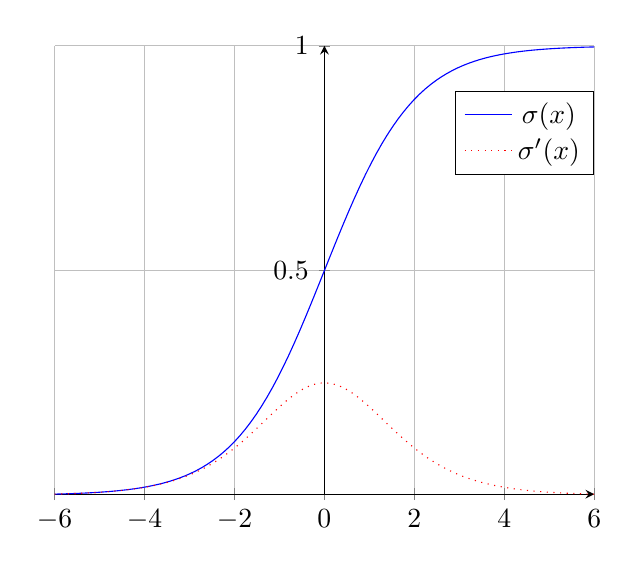
\begin{tikzpicture}[declare function={sigma(\x)=1/(1+exp(-\x));
                  sigmap(\x)=sigma(\x)*(1-sigma(\x));}]
            \begin{axis}%
              [
                grid=major,
                xmin=-6,
                xmax=6,
                axis x line=bottom,
                ytick={0,.5,1},
                ymax=1,
                axis y line=middle,
                samples=100,
                domain=-6:6,
                legend style={at={(1,0.9)}}
              ]
              \addplot[blue,mark=none]   (x,{sigma(x)});
              \addplot[red,dotted,mark=none]   (x,{sigmap(x)});
              \legend{$\sigma(x)$,$\sigma'(x)$}
            \end{axis}
          \end{tikzpicture}
        \end{center}

  \item $\nabla$ 在数学中用于表示向量的微分计算。当 $\nabla$ 应用在一维域的函数上时,即为标准的函数求导;
        当 $\nabla$ 应用在一个场上(也就是多维域),它可能代表着如下三种含义中的一个:
        \begin{enumerate}[i]
          \item 梯度(gradient):$f = \nabla f$
          \item 向量的发散度(divergence):$\textrm{div}\, \overrightarrow{v} = \nabla \cdot \overrightarrow{v}$
          \item 向量的旋度(curl):$\textrm{curl}\, \overrightarrow{v} = \nabla \times \overrightarrow{v}$
        \end{enumerate}
\end{enumerate}

本章其余名词:

\begin{center}
  \begin{tabular}{ |p{4cm}||p{7cm}|  }
    \hline
    \multicolumn{2}{|c|}{\textbf{神经元模型}}               \\
    \hline
    名称       & 英文                                      \\
    \hline
    功能神经元    & functional neuron                       \\
    \hline
    线性可分     & linearly separable                      \\
    \hline
    收敛       & converge                                \\
    \hline
    震荡       & fluctuation                             \\
    \hline
    隐层或隐含层   & hidden layer                            \\
    \hline
    多层前馈神经网络 & multi-layer feedforward neural networks \\
    \hline
    连接权      & connection weight                       \\
    \hline
  \end{tabular}
\end{center}

\newpage

\subsection{误差反向传播算法}

误差反向传播算法(error BackPropagation,简称 BP)。

给定训练集 $D = \{(\pmb{x}_1, \pmb{y}_1), (\pmb{x}_2, \pmb{y}_2),\dots,(\pmb{x}_m, \pmb{y}_m)\},\,
  \pmb{x}_i \in \mathbb{R}^d,\, \pmb{y}_i \in \mathbb{R}^l$,即 input 为 $d$ 维,output $l$ 维。如图:

\begin{center}
  \tikzset{%
    every neuron/.style={
        circle,
        draw,
        minimum size=0.7cm
      },
    neuron missing/.style={
        draw=none,
        scale=2,
        text width=0.444cm,
        execute at begin node=\color{black}$\hdots$
      },
  }

  \begin{tikzpicture}[x=1cm, y=1.5cm, >=stealth]

    % ================================================================================================
    % 神经元
    % ================================================================================================
    \foreach \m [count=\i] in {1,missing,2,missing,3}
    \node [every neuron/.try, neuron \m/.try ] (output-\m) at (\i+2.22,4) {};

    \foreach \m [count=\i] in {1,2,missing,3,missing,4}
    \node [every neuron/.try, neuron \m/.try ] (hidden-\m) at (\i*1.5,2) {};

    \foreach \m [count=\i] in {1,missing,2,missing,3}
    \node [every neuron/.try, neuron \m/.try] (input-\m) at (\i+2.22,0) {};

    % ================================================================================================
    % 神经元标记
    % ================================================================================================
    \foreach \m [count=\i] in {1,j,l}
    \node [above] at (output-\i.north) {$y_\m$};

    \foreach \m [count=\i] in {1,2,h,q}
    \node [above=0.1,right] at (hidden-\i.east) {$b_\m$};

    \foreach \m [count=\i] in {1,i,d}
    \node [below] at (input-\i.south) {$x_\m$};


    % ================================================================================================
    % 注解
    % ================================================================================================
    \draw [red,dashed,->] (output-2) -- ++(0.8,-0.35) -- ++(3.4,0)
    node [below=0.33,right] {\shortstack{第 $j$ 个输出神经元的输入 \\ $\beta_j = \sum\limits_{h=1}^{q} w_{hj}b_h$}};

    \draw [red,dashed,->] (hidden-3) -- ++(0.8,-0.45) -- ++(2.6,0)
    node [below=0.33,right] {\shortstack{第 $h$ 个隐层神经元的输入 \\ $\alpha_j = \sum\limits_{i=1}^{d} v_{ih}x_i$}};

    % ================================================================================================
    % 连接
    % ================================================================================================
    \foreach \i in {1,...,4}
    \foreach \j in {1,3}
    \draw [-] (hidden-\i.north) -- (output-\j.south);

    \foreach \i in {1,...,4}
    \draw [red,-] (hidden-\i.north) -- (output-2.south);

    \foreach \i in {1,...,3}
    \foreach \j in {1,2,4}
    \draw [-] (input-\i.north) -- (hidden-\j.south);

    \foreach \i in {1,...,3}
    \draw [red,-] (input-\i.north) -- (hidden-3.south);

    % ================================================================================================
    % 标记
    % ================================================================================================
    \foreach \m [count=\i] in {1,2,h,q}
    \node [yshift=10,fill=white,text=red,scale=0.8] at (hidden-\i.north) {$w_{\m j}$};

    \foreach \m [count=\i] in {1,i,d}
    \node [yshift=10,fill=white,text=red,scale=0.8] at (input-\i.north) {$v_{\m j}$};

    % ================================================================================================
    % 注解
    % ================================================================================================
    \foreach \l [count=\i from 0] in {输入, 隐, 输出}
    \node [align=center, left] at (0,\i*2) {\l 层};

  \end{tikzpicture}
\end{center}

如图所示,该神经网络是一个拥有 $d$ 个输入神经元,$l$ 个输出神经元,$q$ 个隐层神经元的多层前馈网络结构。
\bigbreak

其中输出层第 $j$ 个神经元的\textcolor{Cerulean}{\textbf{阈值}}用 \textcolor{Cerulean}{$\theta_j$} 表示,
隐层第 $h$ 个神经元的\textcolor{Cerulean}{\textbf{阈值}}用 \textcolor{Cerulean}{$\gamma_h$} 表示;
输入层第 $i$ 个神经元与隐层第 $h$ 个神经元之间的\textcolor{BurntOrange}{\textbf{连接权}}为 \textcolor{BurntOrange}{$v_{ih}$},
隐层第 $h$ 个神经元与输出层第 $j$个神经元之间的\textcolor{BurntOrange}{\textbf{连接权}}为 \textcolor{BurntOrange}{$w_{hj}$}。
\bigbreak

其中隐层的第 $h$ 个神经元接收到的\textcolor{Plum}{\textbf{输入}}
为 \textcolor{Plum}{$\alpha_h = \sum_{i=1}^{d} v_{ih} x_i$}(图中输入层与隐层之间的三条红线所示);
输出层的第 $j$ 个神经元接收到的\textcolor{Plum}{\textbf{输入}}
为 \textcolor{Plum}{$\beta_j = \sum_{h=1}^{q} w_{hj} b_h$}(图中隐层与输出层之间的四条红线所示),
其中 \textcolor{ForestGreen}{$b_h$} 为隐层第 $h$ 个神经元的\textcolor{ForestGreen}{\textbf{输出}}。
\bigbreak

对训练例 $(\pmb{x}_k, \pmb{y}_k)$ 假设神经网络的输出为 $\hat{\pmb{y}}_k = (\hat{y}_1^k,\hat{y}_2^k,\dots,\hat{y}_l^k,)$,即
\begin{equation}
  \hat{y}_j^k = f(\beta_j - \theta_j)
\end{equation}

这里的真实值 $y_j^k = (y_1^k,y_2^k,\dots,y_l^k)^2$,那么对于某第 i 个输出层的神经元而言,其均方误差即
\[
  \frac{(\hat{y}_i^k - y_i^k)}{2}
\]
那么将所有神经元加总,就有了网络在 $(\pmb{x}_k, \pmb{y}_k)$ 上的均方误差为:
\begin{equation}
  E_k = \frac{1}{2} \sum_{j=1}^{l} (\hat{y}_j^k - y_j^k)^2
\end{equation}

另外上图的网络中有 $(d + l + l) q + l$ 个参数需确定:输入层到隐层的 $d \times q$ 个权值、隐层到输出层的 $q \times l$ 个权值、
$q$ 个隐层神经元的阈值、$l$ 个输出层神经元的阈值。BP 是一个迭代学习算法,在迭代的每一轮中采用广义的感知机学习规则对参数进行更新估计,
即与式 5.1 类似,任意参数 $v$ 的更新估计式为
\begin{equation}
  v \leftarrow v + \Delta v.
\end{equation}

BP 算法基于 \textbf{梯度下降(gradient descent)} 策略,以目标的\textit{负}梯度方向\textit{对参数进行调整}。
对式 5.4 的误差 $E_k$,给定学习率 $\eta$,有
\begin{equation}
  \Delta w_{hj} = -\eta \frac{\partial E_k}{\partial w_{hj}}
\end{equation}

这里提到的负梯度,是利用了导数趋近于零时可以得到最小值的特性,去求得均方误差 $E_k$ 的最小值。回顾上文中的感知机学习算法:
\begin{aquote}
  ...随机选取一个误分类点并使其梯度下降,所以权重 $\pmb{w}$ 的更新式为
  \begin{gather*}
    \pmb{w} \leftarrow \pmb{w} + \Delta \pmb{w}, \\
    \Delta \pmb{w} = -\eta (\hat{y}_i - y_i) \pmb{w} = \eta (y_i - \hat{y}_i) \pmb{w}
  \end{gather*}
\end{aquote}

式 5.6 与感知机的最小化损失函数的不同之处在于:感知机是有两层神经元构成的,且输出层只有一个神经元,因此只需要考虑一层的权重变化,
即 $(\hat{y}_i - y_i) \pmb{w}$;而对于由若干个感知机所构成的神经网络而言,所有权重的变化则变为了
$\frac{\partial E_k}{\partial w_{hj}}$。

那么对于多层的神经网络,式 5.4 仅表现出了最后一层隐层与输出层的权重变化,那么就有了疑问:其它层之间的权重好像并不会被式 5.6 所改变?
我们接着往下看,注意到 $w_hj$ 先影响到第 $j$ 个输出层神经元的输入值 $\beta_j$。根据图示其为隐层所有神经元与其本身的表达式,即
\[ \beta_j = \sum_{h=1}^{q} w_{hj} b_h \]
接着 $w_{hj}$ 再影响到其他输出值 $\hat{y}_j^k$,最后再影响到 $E_k$,那么根据求导的链式法则有:
\begin{equation}
  \frac{\partial E_k}{\partial w_{hj}} =
  \frac{\partial E_k}{\partial \hat{y}_j^k} \cdot
  \frac{\partial \hat{y}_j^k}{\partial \beta_j} \cdot
  \frac{\partial \beta_j}{\partial w_{hj}}
\end{equation}

根据 $\beta_j$ 的定义,有:
\begin{equation}
  \begin{split}
    \frac{\partial \beta_j}{\partial w_{hj}} & = \frac{\partial (\sum_{h=1}^{q} w_{hj} b_h) }{\partial w_{hj}} \\
    & = \frac{\partial (w_{1j}b_1 + w_{2j}b_2 + \cdots + w_{hj}b_h + \cdots + w_{qj}b_q)}{\partial w_{hj}} \\
    & = 0 + 0 + \cdots + b_h + \cdots + 0 \\
    & = b_h
  \end{split}
\end{equation}

而又根据 Sigmoid 函数的一个很好的性质:
\begin{equation}
  f'(x) = f(x)(1 - f(x))
\end{equation}

根据式 5.4 与式 5.3 有:
\begin{equation}
  \begin{split}
    g_j & = -\frac{\partial E_k}{\partial \hat{y}_j^k} \cdot \frac{\partial \hat{y}_j^k}{\partial \beta_j} \\
    & = -(\hat{y}_j^k - y_j^k)f'(\beta_j - \theta_j) \\
    & = \hat{y}_j^k (1 - \hat{y}_j^k)(y_j^k - \hat{y}_j^k)
  \end{split}
\end{equation}

将式 5.10 与式 5.8 代入式 5.7,再代入式 5.6,就得到了 BP 算法中关于 $w_{hj}$ 的更新公式:
\begin{equation}
  \begin{split}
    \Delta w_{hj} & = -\eta \frac{\partial E_k}{\partial w_{hj}} \\
    & = -\eta \frac{\partial E_k}{\partial \hat{y}_j^k} \cdot
    \frac{\partial \hat{y}_j^k}{\partial \beta_j} \cdot
    \frac{\partial \beta_j}{\partial w_{hj}} \\
    & = \eta \hat{y}_j^k (1 - \hat{y}_j^k)(y_j^k - \hat{y}_j^k) \cdot b_h \\
    & = \eta g_j b_h
  \end{split}
\end{equation}

类似可得:
\begin{equation}
  \Delta \theta_j = -\eta g_j
\end{equation}
\begin{equation}
  \Delta v_{ih} = \eta e_h x_i
\end{equation}
\begin{equation}
  \Delta \gamma_h = -\eta e_h
\end{equation}

式 5.13 与 5.14 中

\begin{equation}
  \begin{split}
    e_n & = -\frac{\partial E_k}{\partial b_h} \cdot \frac{\partial b_h}{\partial \alpha_h} \\
    & = -\sum_{j=1}^{i} \frac{\partial E_k}{\partial \beta_j} \cdot \frac{\partial \beta_j}{\partial b_h} f'(\alpha_h - \gamma_h) \\
    & = \sum_{j=1}^{l} w_{hj} g_j f'(\alpha_h - \gamma_h) \\
    & = b_h (1 - b_h) \sum_{j=1}^{l} w_{hj} g_j
  \end{split}
\end{equation}

\bigbreak
\textbf{式 5.12 解析}

因为:

\[
  \Delta \theta_j = -\eta \frac{\partial E_k}{\partial \theta_j}
\]

同时有:

\begin{align*}
  \begin{split}
    \frac{\partial E_k}{\partial \theta_j} & = \frac{\partial E_k}{\partial \hat{y}_j^k} \cdot
    \frac{\partial \hat{y}_j^k}{\partial \theta_j} \\
    & = \frac{\partial E_k}{\partial \hat{y}_j^k} \cdot
    \frac{\partial [f(\beta_j - \theta_j)]}{\partial \theta_j} \\
    & = \frac{\partial E_k}{\partial \hat{y}_j^k} \cdot
    f'(\beta_j - \theta_j) \times (-1) \\
    & = \frac{\partial E_k}{\partial \hat{y}_j^k} \cdot
    f(\beta_j - \theta_j) \times [1 - f(\beta_j - \theta_j)] \times (-1) \\
    & = \frac{\partial E_k}{\partial \hat{y}_j^k} \cdot
    \hat{y}_j^k (1 - \hat{y}_j^k) \times (-1) \\
    & = \frac{\partial [\frac{1}{2} \sum_{j=1}^{l} (\hat{y}_j^k - y_j^k)^2]}{\partial \hat{y}_j^k} \cdot
    \hat{y}_j^k (1 - \hat{y}_j^k) \times (-1) \\
    & = \frac{1}{2} \times 2(\hat{y}_j^k - y_j^k) \times 1 \cdot \hat{y}_j^k (1 - \hat{y}_j^k) \times (-1) \\
    & = (\hat{y}_j^k - y_j^k) \hat{y}_j^k (1 - \hat{y}_j^k) \\
    & = g_j
  \end{split}
\end{align*}

所以:

\[
  \Delta \theta_j = -\eta g_j = -\eta \frac{\partial E_k}{\partial \theta_j}
\]

\textbf{式 5.13 解析}

因为:

\[
  \Delta v_{ih} = -\eta \frac{\partial E_k}{\partial v_{ih}}
\]

同时有:

\begin{align*}
  \begin{split}
    \frac{\partial E_k}{\partial v_{ih}} & = \sum_{j=1}^{l} \frac{\partial E_k}{\partial \hat{y}_j^k} \cdot
    \frac{\partial \hat{y}_j^k}{\partial \beta_j} \cdot \frac{\partial \beta_j}{\partial b_h} \cdot
    \frac{\partial b_h}{\partial \alpha_h} \cdot \frac{\partial \alpha_h}{\partial v_ih} \\
    & = \sum_{j=1}^{l} \frac{\partial E_k}{\partial \hat{y}_j^k} \cdot
    \frac{\partial \hat{y}_j^k}{\partial \beta_j} \cdot \frac{\partial \beta_j}{\partial b_h} \cdot
    \frac{\partial b_h}{\partial \alpha_h} \cdot x_i \\
    & = \sum_{j=1}^{l} \frac{\partial E_k}{\partial \hat{y}_j^k} \cdot
    \frac{\partial \hat{y}_j^k}{\partial \beta_j} \cdot \frac{\partial \beta_j}{\partial b_h} \cdot
    f'(\alpha_h - \gamma_h) \cdot x_i \\
    & = \sum_{j=1}^{l} \frac{\partial E_k}{\partial \hat{y}_j^k} \cdot
    \frac{\partial \hat{y}_j^k}{\partial \beta_j} \cdot w_{hj} \cdot f'(\alpha_h - \gamma_h) \cdot x_i \\
    & = \sum_{j=1}^{l} (-g_j) \cdot w_{hj} \cdot f'(\alpha_h - \gamma_h) \cdot x_i \\
    & = - f'(\alpha_h - \gamma_h) \cdot \sum_{j=1}^{l} (g_j) \cdot w_{hj} \cdot x_i \\
    & = - b_h (1 - b_h) \cdot \sum_{j=1}^{l} (g_j) \cdot w_{hj} \cdot x_i \\
    & = - e_h \cdot x_i
  \end{split}
\end{align*}

所以:

\[
  \Delta v_{ih} = -\eta \frac{\partial E_k}{\partial v_{ih}} = \eta e_h x_i
\]

\textbf{式 5.14 解析}

因为:

\[
  \Delta \gamma_h = -\eta \frac{\partial E_k}{\partial \gamma_h}
\]

同时有:

\begin{align*}
  \begin{split}
    \frac{\partial E_k}{\partial \gamma_h} & = \sum_{j=1}^{l} \frac{\partial E_k}{\partial \hat{y}_j^k} \cdot
    \frac{\partial \hat{y}_j^k}{\partial \beta_j} \cdot \frac{\partial \beta_j}{\partial b_h} \cdot
    \frac{\partial b_h}{\partial \gamma_h} \\
    & = \sum_{j=1}^{l} \frac{\partial E_k}{\partial \hat{y}_j^k} \cdot
    \frac{\partial \hat{y}_j^k}{\partial \beta_j} \cdot \frac{\partial \beta_j}{\partial b_h} \cdot
    f'(\alpha_h - \gamma_h) \cdot (-1) \\
    & = -\sum_{j=1}^{l} \frac{\partial E_k}{\partial \hat{y}_j^k} \cdot
    \frac{\partial \hat{y}_j^k}{\partial \beta_j} \cdot w_{hj} \cdot f'(\alpha_h - \gamma_h) \\
    & = -\sum_{j=1}^{l} \frac{\partial E_k}{\partial \hat{y}_j^k} \cdot
    \frac{\partial \hat{y}_j^k}{\partial \beta_j} \cdot w_{hj} \cdot b_h (1 - b_h) \\
    & = \sum_{j=1}^{l} g_j \cdot w_{hj} \cdot b_h (1 - b_h) \\
    & = e_h
  \end{split}
\end{align*}

所以:

\[
  \Delta \gamma_h = -\eta \frac{\partial E_k}{\partial \gamma_h} = -\eta e_h
\]

\newpage
\textbf{BP 算法的工作流程}:

\begin{shaded}
  \textbf{输入}:

  训练集 $D = \{(\pmb{x}_k, \pmb{y_k})\}_{k=1}^m$;

  学习率 $\eta$.
  \bigskip

  \textbf{过程}:

  1: 在 $(0,1)$ 范围内随机初始化网络中所有连接权和阈值

  2: \textbf{repeat}

  3. \aidnt \textbf{for all} $(\pmb{x}_k, \pmb{y}_k) \in D$ \textbf{do}

  4. \aidnt[2] 根据当前参数和式 5.3 计算当前样本的输出 $\hat{\pmb{y}}_k$;
  \[ \hat{y}_j^k = f(\beta_j - \theta_j) \]

  5. \aidnt[2] 根据式 5.10 计算输出层神经元的梯度项 $g_j$;
  \[ g_j = \hat{y}_j^k (1 - \hat{y}_j^k) (y_j^k - \hat{y}_j^k) \]

  6. \aidnt[2] 根据式 5.15 计算隐层神经元的梯度项 $e_h$;
  \[ e_h = b_h (1 - b_h) \sum_{j=1}^{l} w_{hj} g_j \]

  7. \aidnt[2] 根据式 5.11 - 5.14 更新连接权 $w_{hj},\ v_{ih}$ 与阈值 $\theta_j,\ \gamma_h$
  \begin{equation*}
    \begin{cases}
      \Delta w_{hj} = \eta g_j b_h \\
      \Delta \theta_j = -\eta g_j  \\
      \Delta v_{ih} = \eta e_h x_i \\
      \Delta \gamma_h = -\eta e_h
    \end{cases}
  \end{equation*}

  8. \aidnt \textbf{end for}

  9. \textbf{until} 达到停止条件

  \textbf{输出}:连接权与阈值确定的多层前馈神经网络
\end{shaded}

需要注意,BP 算法的目标是要最小化训练集 $D$ 上的累积误差($m$ 即训练集的样本个数)
\begin{equation}
  E = \frac{1}{m} \sum_{k=1}^{m} E_k
\end{equation}

但是上面介绍的“标准BP算法”每次仅针对一个训练样例更新连接权和阈值,意味着上述工作流程中的更新规则是基于单个 $E_k$ 推导而得。
如果类似推导出基于累积误差最小化的更新规则,那么就得到了\textbf{累积误差反向传播(accumulated error backpropagation)}
算法。

\bigbreak
那么来比较一下两种算法的差异:

\begin{center}
  \begin{tabular}{ |p{2cm}||p{5cm}|p{5cm}|  }
    \hline
    \multicolumn{3}{|c|}{\textbf{BP 算法}}                     \\
    \hline
    差异   & 标准 BP 算法                 & 累积 BP 算法               \\
    \hline
    参数更新 & 只针对单个样例                  & 直接针对累积误差最小化            \\
    \hline
    更新频率 & 非常频繁,且对不同样例进行更新可能会出现“抵消” & 很低,因为是读取整个训练集后才对参数进行更新 \\
    \hline
    迭代次数 & 多                        & 少                      \\
    \hline
    类比   & 随机梯度下降                   & 标准梯度下降                 \\
    \hline
  \end{tabular}
\end{center}

注:随机梯度下降(stochastic gradient descent)
在训练集非常大时,累积误差下降到一定程度后,进一步下降会非常缓慢,这时切换为标准 BP 可以更快获得较好的解。

两种策略来缓解 BP 网络的过拟合:
\begin{enumerate}
  \item \textbf{早停(early stopping)}:将数据分成训练集和验证集,训练集用来计算梯度、更新连接权和阈值,验证集用来估计误差,
        若训练集误差降低但验证集误差升高,则停止训练,同时返回具有最小验证集误差的连接权和阈值。
  \item \textbf{正则化(regularization)}:在误差目标函数中增加一个用于描述网络复杂度的部分,例如连接权与阈值的平方和。
        仍然令 $E_k$ 表示第 $k$ 个训练样例上的误差,$w_i$ 表示连接权和阈值,则误差目标函数 5.16 变为
        \begin{equation}
          E = \lambda \frac{1}{m} \sum_{k=1}^{m} E_k + (1-\lambda) \sum_{i} w_i^2
        \end{equation}
        其中 $\lambda \in (0,1)$ 用于对经验误差与网络复杂度这两项进行折中,通常会使用交叉验证法来估计。
\end{enumerate}

注:引入正则化策略的神经网络与第 6 章的 SVM 非常相似。

\newpage
\textbf{补充}

BP 算法的计算流程。

\begin{itemize}
  \item $x$ 输入,即特征向量;
  \item $y$ 目标输出。对于分类问题而言,输出是一个类型概率的向量(例 $(0.1, 0.7, 0.2)$),而目标输出是某个特定的类型,
        由 one-hot/dummy variable 编码(例 $(0, 1, 0)$);
  \item $C$ 损失函数或代价函数。对于分类问题而言,这通常是交叉熵 cross entropy(XC),而对回归问题而言则是平方错误损失
        squared error loss(SEL);
  \item $L$ 神经网络的层数;
  \item $W^l = (w_{jk}^l$ 神经网络中 $l-1$ 层与 $l$ 层之间的权重,而 $w_{jk}^l$ 则是在 $l-1$ 层的第 $k$ 个节点
        与 $l$ 层第 $j$ 个节点之间的权重;
  \item $f^l$ 神经网络中 $l$ 层的激活函数。对于分类问题,二元分类的最后一层通常是对数函数,多种类分类则是 softmax 函数,
        而传统做法中,隐层的节点通常是 sigmoid 函数,今天更多样化了,线性整流函数 rectified 更为普遍(ramp,ReLU)。
\end{itemize}

整个网络实际上是一个关于\textbf{函数组合 function composition} 与\textbf{矩阵乘法 matrix multiplication} 的结合:

\[
  g(x) := f^L (W^L f^{L-1}(W^{L-1} \cdots f^1(W^1x) \cdots))
\]

对于训练集而言,输入-输出对 $\{(x_i, y_i)\}$ 视为一个集;而模型在每个输入-输出对 $(x_i, y_i)$ 的损失实际上是预测值 $g(x_i)$
与目标输出 $y_i$ 的差异:
\[ C(y_i, g(x_i)) \]

注意这里的差异:在模型评估时,权重是固定的,而输入是变化的(且目标输出可能是不可知的),此时神经网络结束于输出层(它并不包含损失函数);
而在模型训练时,输入-输出对是固定的,而权重是变化的,此时神经网络结束于损失函数。

反向传递计算出固定的输入-输出对 $(x_i, y_i)$ 的梯度,其中权重 $w_{jk}^l$ 是可变的。每个独立的梯度 $\partial C/\partial w_{jk}^l$
可以被链式计算;而分开计算每个权重是低效的。反向传递通过避免重复计算以及不去计算非必要的中间值,从而可以高效的计算出梯度,即计算每层的
梯度 -- 具体而言,是从后向前的,每层加权输入的梯度,以 $\delta^l$ 表示。

这里的关键点在于,在 $W^l$ 中的权重影响损失是通过它在下一层的作用,又因为整个过程是线性的,$\delta^l$ 是唯一一个在 $l$ 层中
需要计算的数据,有此可以计算上一层 $\delta^{l-1}$ 并递归下去。这样就在两个层面避免了低效:首先,它避免了重复,因为当计算 $l$ 层
的梯度时,不需要每次都重新计算之后所有 $l+1, l+2$ 层的导数;其次,它避免了非必要的中间计算,因为每个阶段它直接计算了最终输出(损失)
权重的梯度,而不是不必要的计算隐层中关于权重变化 $\partial a_{j'}^{l'} / \partial w_{jk}^l$ 数值的导数。


\begin{enumerate}[I]
  \item \textbf{矩阵乘法}

        给定一个输入-输出对 $(x,y)$,其损失为:
        \[ C(y, f^L(W^L f^{L-1}(W^{L-1} \cdots f^2(W^2 f^1(W^1 x)) \cdots))) \]

        计算损失首先从输入 $x$ 开始并前向进行;将每个隐层的加权输入表示为 $z^l$,同时将隐层 $l$ 的输出记为激活 $a^l$。
        对于反向传播,激活 $a^l$ 以及导数 $(f^l)'$(在 $z^l$ 计算)必须被缓存。

        关于输入的损失导数由链式法则给出;注意每一项都是\href{https://en.wikipedia.org/wiki/Total_derivative}{\textbf{全微分}},
        计算在神经网络(每个节点)的值:
        \[
          \frac{dC}{da^L} \circ \frac{da^L}{dz^L} \cdot \frac{dz^L}{da^{L-1}} \circ \frac{da^{L-1}}{dz^{L-1}}
          \cdot \frac{dz^{L-1}}{da^{L-2}} \circ \cdots \circ \frac{da^1}{dz^1} \cdot
          \frac{\partial z^1}{\partial x}
        \]

        \begin{itemize}
          \item [\textit{注1}]
                函数 $f$ 在某一点的全微分是指该函数在该点附近关于其自变量的最佳线性近似;与偏微分不同,
                全微分反映了函数关于其所有自变量的线性近似,而非单个自变量。
                \[ f(x) = \int_0^x f'(t) dt \]
          \item [\textit{注2}]
                对于组合函数 $g \circ f$ 在 $a$ 的全微分,满足链式法则:
                \[ d(g \circ f)_a = dg_{f(a)} \cdot df_a \]
          \item [\textit{注3}]
                这里的 $\circ$ 为 \href{https://en.wikipedia.org/wiki/Hadamard_product_(matrices)}{Hadamard product},
                即元素一一相乘。
        \end{itemize}

        这些项分别为:损失函数的导数;激活函数的导数;以及矩阵的权重:
        \[
          \frac{dC}{da^L} \circ (f^L)' \cdot W^L \circ (f^{L-1}) \circ \cdots \circ (f^l)' \cdot W^l
        \]

        梯度 $\nabla$ 是输出(由输入表示的)的导数转置,因此矩阵式转置的,且乘法的顺序是相反的,但是入口是一致的:
        \[
          \nabla_x C = (W^{-1}) \cdot (f^1)' \circ \cdots \circ (W^{L-1})^T \cdot (f^{L-1})' \circ (W^L)^T
          \cdot (f^L)' \circ \nabla_{a^L} C
        \]

        反向传播则是该表达式,从右向左计算所构成的(相当于从左到右乘上前一个表达式的导数),有此计算每一次的梯度;另外还有额外的一步加法,
        这是因为权重的梯度不仅仅是一个子表达式:还有一步额外的乘法。

        对于部分乘积(从右至左)的辅助值 $\delta^l$,表述为“$l$ 层的错误”,且定义 $l$ 层输入值的梯度:
        \[
          \delta^l := (f^l)' \circ (W^{l+1})^T \circ \cdots \circ (W^{L-1})^T \cdot (f^{L-1})' \circ (W^L)^T
          \cdot (f^L)' \circ \nabla_{a^L} C
        \]

        注意 $\delta^l$ 是一个向量,其长度是 $l$ 层神经元的数量;每部分都被表述为“该节点的损失属性”

        那么 $l$ 层权重的梯度则为:
        \[ \nabla_{W^l} C = \delta^l (a^{l-1})^T \]

        这里的 $a^{l-1}$ 是因为在 $l-1$ 与 $l$ 层直接的权重 $W^l$ 按比例影响 $l$ 层的输入(激活):输入是固定的,权重是可变的。

        那么 $\delta$ 就可以很容易的递归计算出来,从右至左:
        \[ \delta^{l-1} := (f^{l-1})' \circ (W^l)^T \cdot \delta^l \]

        那么权重的梯度可以通过每层的矩阵乘法而计算出来;这便是反向传播。

  \item \textbf{导数}
        注:以下资料以另一个角度来解读式 5.11。

        梯度下降方法牵涉到计算损失函数相对于网络权重的导数。这通常是通过反向传播算法完成的。假设一个输出神经元,有方差函数
        \[ E = L(t, y) \]
        其中
        \begin{itemize}
          \item $L$ 是输出 $y$ 与目标值 $t$ 的损失;
          \item $t$ 是训练样本的目标输出;
          \item $y$ 是输出神经元的实际输出。
        \end{itemize}

        对于每个神经元 $j$,其输出 $O_j$ 被定义为
        \[ o_j = \varphi(\mathrm{net}_j) = \varphi \Biggl(\sum_{k=1}^{n} w_{kj} x_k\Biggr) \]
        其中激活函数 $\varphi$ 是非线性的,同时在激活区域是可微的(ReLU 在一个点上不可微)。经典的激活函数是对数函数:
        \[ \varphi = \frac{1}{1 + e^{-x}} \]
        其可以方便的进行求导:
        \[ \frac{d \varphi(z)}{dz} = \varphi(z)(1 - \varphi(z)) \]

        这里一个神经元的输入 $\mathrm{net}_j$ 是前一层神经元们输出 $o_k$ 加权之和。如果神经元在神经网络输入层之后的第一层,
        那么输入层的 $o_k$ 即为神经网络的输入 $x_k$。神经元的输入单元数量是 $n$。变量 $w_{kj}$ 表示前一层中神经元 $k$ 与
        当前层神经元 $j$ 之间的权重。

        \textbf{求误差的导数}

        计算误差相对于权重 $w_{ij}$ 的偏微分是通过两次链式法则:
        \begin{equation}
          \frac{\partial E}{\partial w_{ij}} = \frac{\partial E}{\partial o_j} =
          \frac{\partial E}{\partial o_j} \frac{\partial o_j}{\partial\mathrm{net}_j}
          \frac{\partial \mathrm{net}_j}{\partial w_{ij}}
          \tag{I}
        \end{equation}
        上述表达式右侧的最后一个元素,仅有一项在 $\mathrm{net}_j$ 之和中依赖 $w_{ij}$,因此有
        \begin{equation}
          \frac{\partial E}{\partial w_{ij}} = \frac{\partial}{\partial w_{ij}}
          \Biggl(\sum_{k=1}^{n} w_{ki} o_k\Biggr) = \frac{\partial}{\partial w_{ij}} w_{ij} o_i = o_i
          \tag{II}
        \end{equation}

        如果神经元在输出层之后的一层,那么 $o_i$ 就是 $x_i$。

        神经元 $j$ 的输出相对于其输入的倒数就是一个简单的激活函数导数:
        \begin{equation}
          \frac{\partial o_j}{\partial\mathrm{net}_j}=\frac{\varphi(\mathrm{net}_j)}{\partial\mathrm{net}_j}
          \tag{III}
        \end{equation}

        而对于对数激活函数而言有
        \[
          \frac{\partial o_j}{\partial\mathrm{net}_j}=\frac{\partial}{\partial\mathrm{net}_j}\varphi(\mathrm{net}_j)=
          \varphi(\mathrm{net}_j)(1-\varphi(\mathrm{net}_j))=o_j(1-o_j)
        \]
        这也是为什么反向传播需要激活函数是可微的。(尽管如此,ReLU 激活函数,在 0 处并不可微,如今更加普遍,例如在 AlexNet 中)。
        注:\href{https://en.wikipedia.org/wiki/AlexNet}{AlexNet},即 CNN 架构,卷积神经网络。

        如果神经元位于输出层,那么计算很简单,因为 $o_j = y$:
        \begin{equation}
          \frac{\partial E}{\partial o_j} = \frac{\partial E}{\partial y}
          \tag{IV}
        \end{equation}
        如果平方差用作于损失函数,那么可以重写为
        \[
          \frac{\partial E}{\partial o_j} = \frac{\partial E}{\partial y} =
          \frac{\partial}{\partial y} \frac{1}{2} (1-y)^2 = y - t
        \]

        然而,如果 $j$ 是神经网络中隐层中的神经元,那么寻找 $E$ 相对于 $o_j$ 的导数就没那么明显了。
        将 $E$ 视为一个由神经元 $j$ 的得到的输入为全部神经元 $L = \{u,v,\dots,w\}$ 的函数:
        \[
          \frac{\partial E(o_j)}{\partial o_j} =
          \frac{\partial E(\mathrm{net}_u,\mathrm{net}_v,\dots,\mathrm{net}_w)}{\partial o_j}
        \]
        求相对于 $o_j$ 的全微分,那么就得到了一个导数的递归表达式:
        \begin{equation}
          \frac{\partial E}{\partial o_j} =
          \sum_{t \in L}\Biggl(\frac{\partial E}{\partial\mathrm{net}_t}\frac{\partial\mathrm{net}_t}{\partial o_j}\Biggr)=
          \sum_{t \in L}
          \Biggl(
          \frac{\partial E}{\partial o_t}\frac{\partial o_t}{\partial\mathrm{net}_t}\frac{\partial\mathrm{net}_t}{\partial o_j}
          \Biggr)=
          \sum_{t \in L}\Biggl(\frac{\partial E}{\partial o_t}\frac{\partial o_t}{\partial\mathrm{net}_t}w_{jl}\Biggr)
          \tag{V}
        \end{equation}

        因此,当相对下一层的输出 $o_l$ 全部可微时,那么相对于 $o_j$ 的微分则可被计算。[注意,如果 $L$ 中任何神经元没有连接至神经元 $j$,它们则会
        独立于 $w_{ij}$,同时与和相关的偏微分则会消失为 0]。

        将 (II),(III),(IV),(V) 代入进 (I) 中,获得:
        \begin{align*}
          \begin{split}
            \frac{\partial E}{\partial w_{ij}} & = \frac{\partial E}{\partial o_j} \frac{\partial o_j}{\partial\mathrm{net}_j}
            \frac{\partial\mathrm{net}_j}{\partial w_{ij}} \\
            & = \frac{\partial E}{\partial o_j} \frac{\partial o_j}{\partial\mathrm{net}_j} o_i \\
            & = o_i \delta_j
          \end{split}
        \end{align*}
        这其中
        \[
          \delta_j = \frac{\partial E}{\partial o_j} \frac{\partial o_j}{\partial\mathrm{net}_j} =
          \begin{cases}
            \frac{\partial L(o_j,t)}{\partial o_j}      \frac{d\varphi(\mathrm{net}_j)}{d\mathrm{net}_j} & \text{如果 $j$ 是一个输出层的神经元,} \\
            (\sum_{l \in L} w_{jl} \delta_j) \frac{d\varphi(\mathrm{net}_j)}{d\mathrm{net}_j}            & \text{如果 $j$ 是一个隐层的神经元。}
          \end{cases}
        \]
        如果 $\varphi$ 是一个对数函数,那么误差则为平方差:
        \[
          \delta_j = \frac{\partial E}{\partial o_j} \frac{\partial o_j}{\partial\mathrm{net}_j} =
          \begin{cases}
            (o_j - t_j) o_j (1 - o_j)                      & \text{如果 $j$ 是一个输出层的神经元} \\
            (\sum_{l \in L} w_{jl} \delta_j) o_j (1 - o_j) & \text{如果 $j$ 是一个隐层的神经元}
          \end{cases}
        \]

        通过梯度下降法来更新权重 $w_{ij}$,那么就必须选择一个学习率,$\eta > 0$。根据 $w_{ij}$ 的增减,权重的变化必须反应在 $E$ 上。
        如果 $\frac{\partial E}{\partial w_{ij}} > 0$,那么 $w_{ij}$ 增加则 $E$ 增加;相反的,如果 $\frac{\partial E}{\partial w_{ij}} < 0$,
        那么 $w_{ij}$ 增加则 $E$ 减少。新的 $\Delta w_{ij}$ 被添加到就权重上,且学习率与梯度之积再乘上 $-1$ 则能保证 $w_{ij}$ 的变化总是能减少 $E$。
        换言之,下述等式 $-\eta \frac{\partial E}{\partial w_{ij}}$ 总是能在 $w_{ij}$ 改变时令 $E$ 减少:
        \[
          \Delta w_{ij} = -\eta \frac{\partial E}{\partial w_{ij}} = -\eta o_i \delta_j
        \]

  \item \textbf{损失函数}

        损失函数是一个函数,它将一个或多个变量的值映射到一个实数上,直观地表示与这些值相关的一些“成本”。对于反向传播而言,在一个训练样本通过正向传播后,
        损失函数的计算了神经网络输出与期望输出之间的差异。

        损失函数的数学表达式必须满足两个条件,才有可能用于反向传播。首先,对于 $n$ 个独立的训练模型 $x$,可以被写成一个由误差函数 $E_x$ 所构成的均值
        $E = \frac{1}{n} \sum_x E_x$。该假设的原因是,对于单个训练样本,反向传播算法需要计算误差函数的梯度,再被泛化到整个误差函数;其次,它可以
        写成神经网络输出的函数。

\end{enumerate}

\newpage
\subsection{全局最小与局部最小}

WIP

\end{document}
